\begin{figure}[h!]
    \centering
    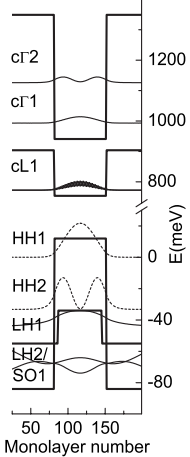
\includegraphics{Images/QWStates.png}
    \caption{Profili degli estremi della banda di valenza e di conduzione. Sono rappresentati i moduli quadri delle funzioni d'onda degli stati confinati degli elettroni e delle lacune. Autostati e autovalori energetici sono stati calcolati a temperatura nulla. Poichè gli spettri sono stati ricavati a temperatura ambiente ci si aspetta una diminuzione del gap interbanda di circa 0.1 eV.}
    \label{fig:my_label}
\end{figure}